\section{Proof the Theorem}
The first direction of \hyperref[thr:kuratowski]{Kuratowski's theorem} states: If graph $G$ contains a subdivision of $K_5$ or $K_{3,3}$ then $G$ is nonplanar

Subdivision of Nonplanar is Nonplanar

If a Subgraph is nonplanar then graph is nonplanar

If a subgraph of graph $G$ is a subdivision of nonplanar then $G$ is nonplanar
\begin{lemma}
    $K_{3,3}$ is nonplanar
\end{lemma}

\begin{proof}
    \begin{figure}[H]
        \begin{minipage}{0.3\textwidth}
            $$V-E+F=2$$
            $$6-E+F=2$$
            $$6-9+F=2$$
            $$F=5$$
        \end{minipage}
        \hfill
        \begin{minipage}{0.35\textwidth}
            \centering
            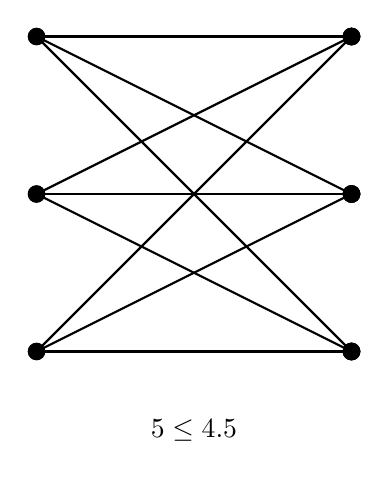
\begin{tikzpicture}
                \foreach \x/\y in {0/1, 0/3, 0/5} {
                        \filldraw[black] (\x,\y) circle (3pt);
                        \foreach \z/\t in {4/1, 4/3, 4/5} {
                                \filldraw[black] (\z,\t) circle (3pt);
                                \draw[black, thick] (\x,\y) -- (\z,\t);
                            }
                    }
                \node at (2,0,0) {$5 \leq 4.5$};
            \end{tikzpicture}
        \end{minipage}
        \hfill
        \begin{minipage}{0.3\textwidth}
            \centering
            No 3 edge faces
            $$4F \leq 2E$$
            $$4F \leq 2 \times 9$$
            $$ F \leq 4.5$$
        \end{minipage}
    \end{figure}
\end{proof}

\begin{lemma}
    $K_5$ is nonplanar
\end{lemma}
\begin{proof}
    \begin{figure}[H]
        \begin{minipage}{0.3\textwidth}
            $$V-E+F=2$$
            $$5-E+F=2$$
            $$5-10+F=2$$
            $$F=7$$
        \end{minipage}
        \hfill
        \begin{minipage}{0.35\textwidth}
            \centering
            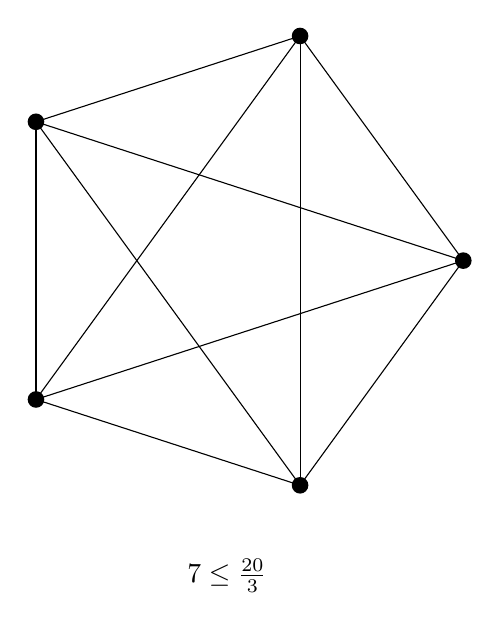
\begin{tikzpicture}
                \foreach \i in {1, 2, 3, 4, 5}
                \fill[black] (\i*360/5:3) coordinate (5\i) circle(3 pt)
                \ifnum \i>1 foreach \j in {\i,...,1}{(5\i) edge (5\j)} \fi;

                \node at (0,-4,0) {$7 \leq \frac{20}{3}$};
            \end{tikzpicture}
        \end{minipage}
        \hfill
        \begin{minipage}{0.3\textwidth}
            \centering
            $$3F \leq 2E$$
            $$3F \leq 2 \times 10$$
            $$F \leq \frac{20}{3}$$
        \end{minipage}
    \end{figure}
\end{proof}
\begin{recap}
    $K_5$ và $K_{3,3}$ are nonplanar

    $\Rightarrow$ All of their subdivisions are nonplanar

    $\Rightarrow$ If graph G contains a subdivision of $K_5$ or $K_{3,3}$ then G is nonplanar
\end{recap}

The second direction of \hyperref[thr:kuratowski]{Kuratowski's theorem} states: If graph $G$ is nonplanar then $G$ contains a subdivision of $K_5$ or $K_{3,3}$
\begin{proof}
    Assume there exist nonplanar graphs which have no subdivisions of $K_5$ or $K_{3,3}$ as subgraphs.

    Let G be the graph of this kind with the $fewest$ edges. Then removing any edge from $G$ gives a $planar$ graph

    \begin{enumerate}
        \item $G$ is 2-connected
              \begin{multicols}{2}
                  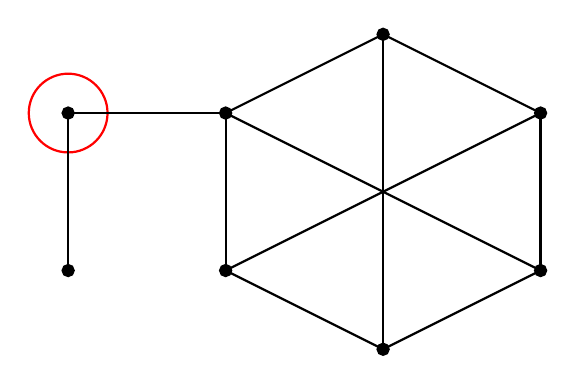
\begin{tikzpicture}
                      \draw[red, thick] (-2,3) circle (0.5);
                      \foreach \x/\y in {0/1, 2/0, 4/1, 0/3, 4/3, 2/4} {
                              \filldraw[black, thick] (\x,\y) circle (2pt);
                              \draw[black, thick] (2,2) -- (\x,\y);
                          }
                      \filldraw[black, thick] (-2,3) circle (2pt);
                      \filldraw[black, thick] (-2,1) circle (2pt);

                      \draw[black, thick] (0,1) -- (2,0);
                      \draw[black, thick] (2,0) -- (4,1);
                      \draw[black, thick] (4,1) -- (4,3);
                      \draw[black, thick] (0,3) -- (0,1);
                      \draw[black, thick] (4,3) -- (2,4);
                      \draw[black, thick] (2,4) -- (0,3);

                      \draw[black, thick] (-2,1) -- (-2,3);
                      \draw[black, thick] (-2,3) -- (0,3);

                  \end{tikzpicture}
              \end{multicols}
        \item $deg(v) \geq 3$ for all vertex $v$ in $G$

              Chứng minh phản chứng: assume some vertex $v \in G$ has $deg(v) \leq 2$

        \item for some $uv \in G$, $G - uv$ is 2-connected

              \begin{tikzpicture}

              \end{tikzpicture}
    \end{enumerate}

\end{proof}

Take the egde $uv$ from the previous statement, and consider the graph $G-uv$ obtained by removing it

$G-uv$ is planar by minimality

$G-uv$ is 2-connected, so there is a cycle contains $u,v$.

\begin{remark}
    Note that the edges we are drawing here are really paths in graph
\end{remark}

\begin{figure}[H]
    \begin{minipage}{0.4\textwidth}
        \begin{tikzpicture}
            \draw[black, thick] (0,0) circle (3);
            \filldraw[black, thick] (-3,0) circle (2pt);
            \filldraw[black, thick] (3,0) circle (2pt);
            \node at (-3.5,0,0) {$u$};
            \node at (3.5,0,0) {$v$};
            \node at (0,2.5,0) {$C$};
        \end{tikzpicture}
    \end{minipage}
    \hfill
    \begin{minipage}{0.5\textwidth}
        Embeded maximal cycle $C$ containing $u,v$
    \end{minipage}

\end{figure}

\begin{figure}[H]
    \begin{minipage}{0.4\textwidth}
        \begin{tikzpicture}
            \draw[black, thick] (0,0) circle (3);
            \filldraw[black, thick] (-3,0) circle (2pt);
            \filldraw[black, thick] (3,0) circle (2pt);
            \node at (-3.5,0,0) {$u$};
            \node at (3.5,0,0) {$v$};
            \node at (0,2.5,0) {$C$};
        \end{tikzpicture}
    \end{minipage}
    \hfill
    \begin{minipage}{0.5\textwidth}
        We embeded $G -uv$ so that $C$ enclose more regions of the graph than any other cycle containing $u$ and $v$ could
    \end{minipage}

\end{figure}

\begin{figure}[H]
    \begin{minipage}{0.4\textwidth}
        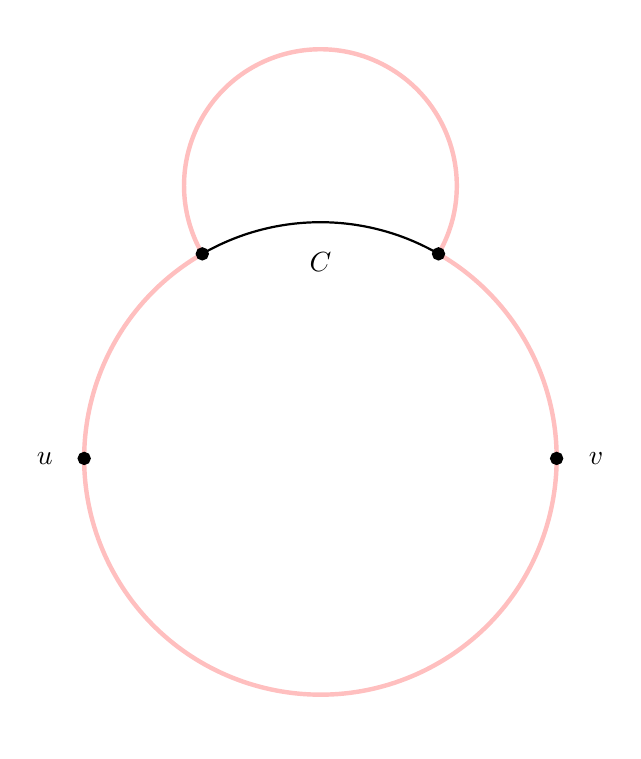
\begin{tikzpicture}
            \draw[pink, ultra thick] (1.5,{sqrt(27/4)}) arc (-30:210:{sqrt(3)});
            \draw[black, thick] (1.5,{sqrt(27/4)}) arc (60:120:3);
            \draw[pink, ultra thick] (-1.5,{sqrt(27/4)}) arc (120:420:3);
            \filldraw[black, thick] (1.5,{sqrt(27/4)}) circle (2pt);
            \filldraw[black, thick] (-1.5,{sqrt(27/4)}) circle (2pt);
            \filldraw[black, thick] (-3,0) circle (2pt);
            \filldraw[black, thick] (3,0) circle (2pt);

            \node at (-3.5,0,0) {$u$};
            \node at (3.5,0,0) {$v$};
            \node at (0,2.5,0) {$C$};
        \end{tikzpicture}
    \end{minipage}
    \hfill
    \begin{minipage}{0.4\textwidth}
        Loop along upper or lower part of $C$?

        We can't have any extra paths on the upper or lower part of $C$ since then there would be a cycle which contains more regions

        Larger cycle $\Rightarrow$ Contradiction
    \end{minipage}

\end{figure}


\begin{figure}[H]
    \begin{minipage}{0.4\textwidth}
        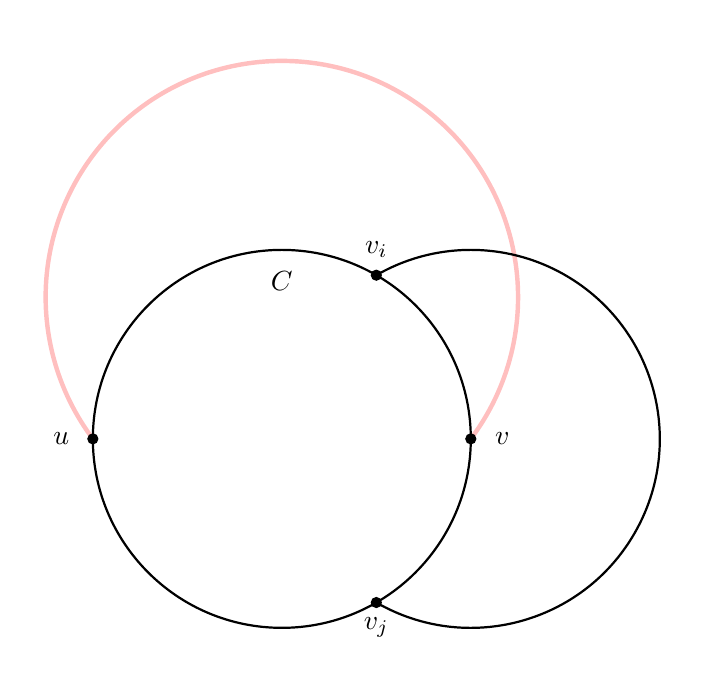
\begin{tikzpicture}[scale = 0.8]
            \draw[black, thick] (0,0) circle (3);
            \draw[pink, ultra thick] (3,0) arc (-acos(3/3.75):180+acos(3/3.75):3.75);
            \draw[black, thick] (1.5,-{sqrt(27/4)}) arc (-120:120:3);

            \filldraw[black, thick] (-3,0) circle (2pt);
            \filldraw[black, thick] (3,0) circle (2pt);
            \filldraw[black, thick] (1.5,{sqrt(27/4)}) circle (2pt);
            \filldraw[black, thick] (1.5,-{sqrt(27/4)}) circle (2pt);
            \node at (1.5,3,0) {$v_i$};
            \node at (1.5,-3,0) {$v_j$};
            \node at (-3.5,0,0) {$u$};
            \node at (3.5,0,0) {$v$};
            \node at (0,2.5,0) {$C$};
        \end{tikzpicture}
    \end{minipage}
    \hfill
    \begin{minipage}{0.4\textwidth}
        $G$ is nonplanar, so we need an osbtruction to $uv$ on the outside of $C$. There must exist a path $v_iv_j$ that blocks $uv$
    \end{minipage}
\end{figure}

The inside of $C$ must contain an obstruction. This obstruction also has to block $v_iv_j$ from being draw inside of $C$ since otherwise we could just draw it inside and draw $uv$ on the outside.

Up to equivalence there are only four types of obstructions we could draw here. \\

\begin{figure}[H]
    \begin{minipage}{0.4\textwidth}
        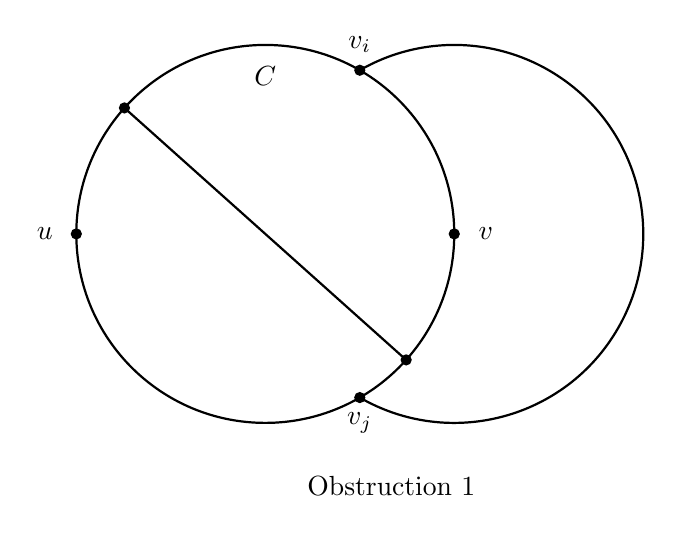
\begin{tikzpicture}[scale = 0.8]
            \draw[black, thick] (0,0) circle (3);
            \draw[black, thick] (1.5,-{sqrt(27/4)}) arc (-120:120:3);
            \draw[black, thick] ({-sqrt(5)},2) -- ({sqrt(5)},-2);
            \filldraw[black, thick] (-3,0) circle (2pt);
            \filldraw[black, thick] (3,0) circle (2pt);
            \filldraw[black, thick] ({-sqrt(5)},2) circle (2pt);
            \filldraw[black, thick] ({sqrt(5)},-2) circle (2pt);
            \filldraw[black, thick] (1.5,{sqrt(27/4)}) circle (2pt);
            \filldraw[black, thick] (1.5,-{sqrt(27/4)}) circle (2pt);
            \node at (1.5,3,0) {$v_i$};
            \node at (1.5,-3,0) {$v_j$};
            \node at (-3.5,0,0) {$u$};
            \node at (3.5,0,0) {$v$};
            \node at (0,2.5,0) {$C$};

            \node at (2,-4,0) {Obstruction 1};
        \end{tikzpicture}
    \end{minipage}
    \hfill
    \begin{minipage}{0.4\textwidth}
        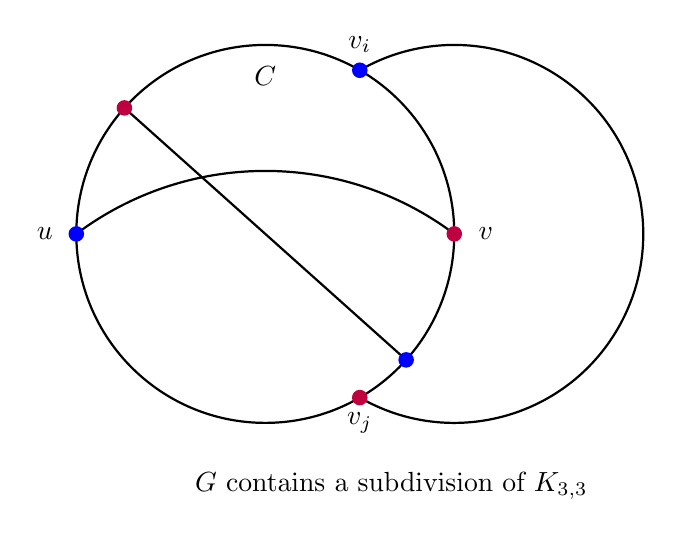
\begin{tikzpicture}[scale = 0.8]
            \draw[black, thick] (0,0) circle (3);
            \draw[black, thick] (1.5,-{sqrt(27/4)}) arc (-120:120:3);
            \draw[black, thick] (3,0) arc (acos(0.6):180-acos(0.6):5);
            \draw[black, thick] ({sqrt(5)},-2) -- (-{sqrt(5)},2);
            \filldraw[blue, thick] (-3,0) circle (3pt);
            \filldraw[purple, thick] (3,0) circle (3pt);
            \filldraw[purple, thick] ({-sqrt(5)},2) circle (3pt);
            \filldraw[blue, thick] ({sqrt(5)},-2) circle (3pt);
            \filldraw[blue, thick] (1.5,{sqrt(27/4)}) circle (3pt);
            \filldraw[purple, thick] (1.5,-{sqrt(27/4)}) circle (3pt);
            \node at (1.5,3,0) {$v_i$};
            \node at (1.5,-3,0) {$v_j$};
            \node at (-3.5,0,0) {$u$};
            \node at (3.5,0,0) {$v$};
            \node at (0,2.5,0) {$C$};
            \node at (2,-4,0) {$G$ contains a subdivision of $K_{3,3}$};

        \end{tikzpicture}
    \end{minipage}
\end{figure}

\begin{figure}[H]
    \begin{minipage}{0.4\textwidth}
        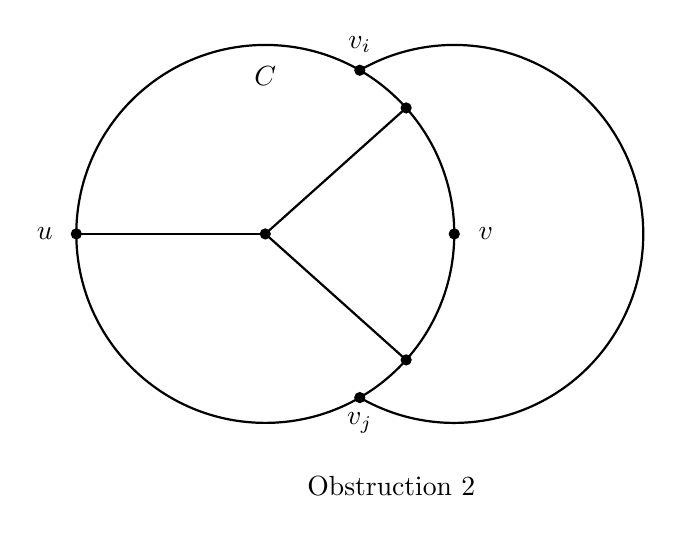
\begin{tikzpicture}[scale = 0.8]
            \draw[black, thick] (0,0) circle (3);
            \draw[black, thick] (1.5,-{sqrt(27/4)}) arc (-120:120:3);
            \draw[black, thick] (0,0) -- ({sqrt(5)},-2);
            \draw[black, thick] (0,0) -- ({sqrt(5)},2);
            \draw[black, thick] (0,0) -- (-3,0);
            \filldraw[black, thick] (-3,0) circle (2pt);
            \filldraw[black, thick] (3,0) circle (2pt);
            \filldraw[black, thick] (0,0) circle (2pt);
            \filldraw[black, thick] ({sqrt(5)},2) circle (2pt);
            \filldraw[black, thick] ({sqrt(5)},-2) circle (2pt);
            \filldraw[black, thick] (1.5,{sqrt(27/4)}) circle (2pt);
            \filldraw[black, thick] (1.5,-{sqrt(27/4)}) circle (2pt);
            \node at (1.5,3,0) {$v_i$};
            \node at (1.5,-3,0) {$v_j$};
            \node at (-3.5,0,0) {$u$};
            \node at (3.5,0,0) {$v$};
            \node at (0,2.5,0) {$C$};

            \node at (2,-4,0) {Obstruction 2};
        \end{tikzpicture}
    \end{minipage}
    \hfill
    \begin{minipage}{0.4\textwidth}
        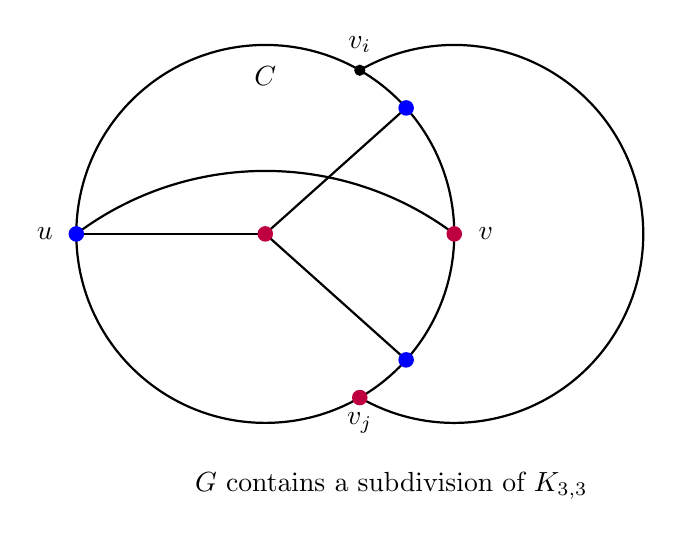
\begin{tikzpicture}[scale = 0.8]
            \draw[black, thick] (0,0) circle (3);
            \draw[black, thick] (1.5,-{sqrt(27/4)}) arc (-120:120:3);
            \draw[black, thick] (3,0) arc (acos(0.6):180-acos(0.6):5);
            \draw[black, thick] (0,0) -- ({sqrt(5)},-2);
            \draw[black, thick] (0,0) -- ({sqrt(5)},2);
            \draw[black, thick] (0,0) -- (-3,0);
            \filldraw[blue, thick] (-3,0) circle (3pt);
            \filldraw[purple, thick] (3,0) circle (3pt);
            \filldraw[purple, thick] (0,0) circle (3pt);
            \filldraw[blue, thick] ({sqrt(5)},2) circle (3pt);
            \filldraw[blue, thick] ({sqrt(5)},-2) circle (3pt);
            \filldraw[black, thick] (1.5,{sqrt(27/4)}) circle (2pt);
            \filldraw[purple, thick] (1.5,-{sqrt(27/4)}) circle (3pt);
            \node at (1.5,3,0) {$v_i$};
            \node at (1.5,-3,0) {$v_j$};
            \node at (-3.5,0,0) {$u$};
            \node at (3.5,0,0) {$v$};
            \node at (0,2.5,0) {$C$};
            \node at (2,-4,0) {$G$ contains a subdivision of $K_{3,3}$};

        \end{tikzpicture}
    \end{minipage}
\end{figure}

\begin{figure}[H]
    \begin{minipage}{0.4\textwidth}
        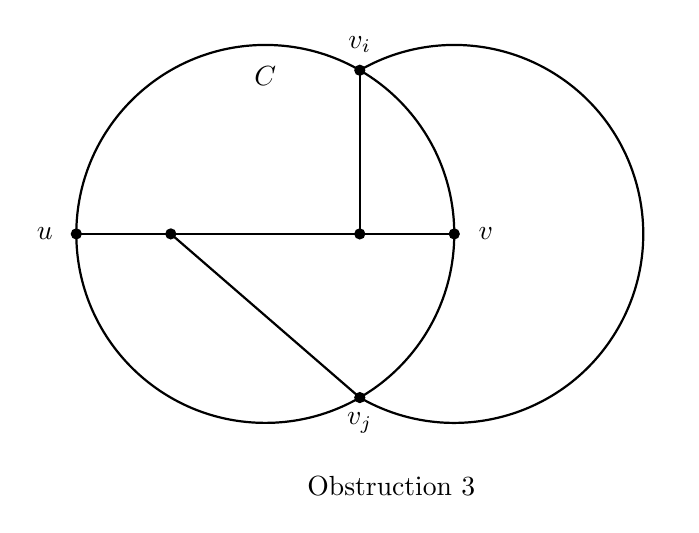
\begin{tikzpicture}[scale = 0.8]
            \draw[black, thick] (0,0) circle (3);
            \draw[black, thick] (1.5,-{sqrt(27/4)}) arc (-120:120:3);
            \draw[black, thick] (3,0) -- (-3,0);
            \draw[black, thick] (1.5,0) -- (1.5,{sqrt(27/4)});
            \draw[black, thick] (-1.5,0) -- (1.5,-{sqrt(27/4)});
            \filldraw[black, thick] (-3,0) circle (2pt);
            \filldraw[black, thick] (3,0) circle (2pt);
            \filldraw[black, thick] (1.5,{sqrt(27/4)}) circle (2pt);
            \filldraw[black, thick] (1.5,-{sqrt(27/4)}) circle (2pt);
            \filldraw[black, thick] (1.5,0) circle (2pt);
            \filldraw[black, thick] (-1.5,0) circle (2pt);
            \node at (1.5,3,0) {$v_i$};
            \node at (1.5,-3,0) {$v_j$};
            \node at (-3.5,0,0) {$u$};
            \node at (3.5,0,0) {$v$};
            \node at (0,2.5,0) {$C$};

            \node at (2,-4,0) {Obstruction 3};
        \end{tikzpicture}
    \end{minipage}
    \hfill
    \begin{minipage}{0.4\textwidth}
        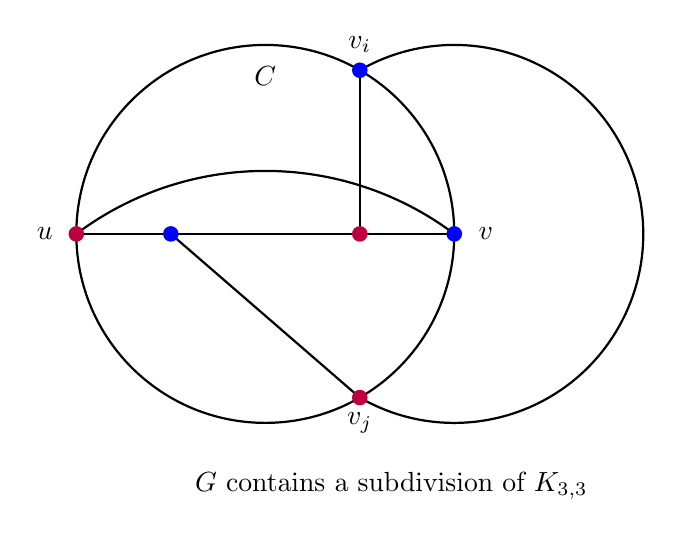
\begin{tikzpicture}[scale = 0.8]
            \draw[black, thick] (3,0) arc (acos(0.6):180-acos(0.6):5);
            \draw[black, thick] (0,0) circle (3);
            \draw[black, thick] (1.5,-{sqrt(27/4)}) arc (-120:120:3);
            \draw[black, thick] (3,0) -- (-3,0);
            \draw[black, thick] (1.5,0) -- (1.5,{sqrt(27/4)});
            \draw[black, thick] (-1.5,0) -- (1.5,-{sqrt(27/4)});
            \filldraw[purple, thick] (-3,0) circle (3pt);
            \filldraw[blue, thick] (3,0) circle (3pt);
            \filldraw[blue, thick] (1.5,{sqrt(27/4)}) circle (3pt);
            \filldraw[purple, thick] (1.5,-{sqrt(27/4)}) circle (3pt);
            \filldraw[purple, thick] (1.5,0) circle (3pt);
            \filldraw[blue, thick] (-1.5,0) circle (3pt);
            \node at (1.5,3,0) {$v_i$};
            \node at (1.5,-3,0) {$v_j$};
            \node at (-3.5,0,0) {$u$};
            \node at (3.5,0,0) {$v$};
            \node at (0,2.5,0) {$C$};
            \node at (2,-4,0) {$G$ contains a subdivision of $K_{3,3}$};

        \end{tikzpicture}
    \end{minipage}
\end{figure}


\begin{figure}[H]
    \begin{minipage}{0.4\textwidth}
        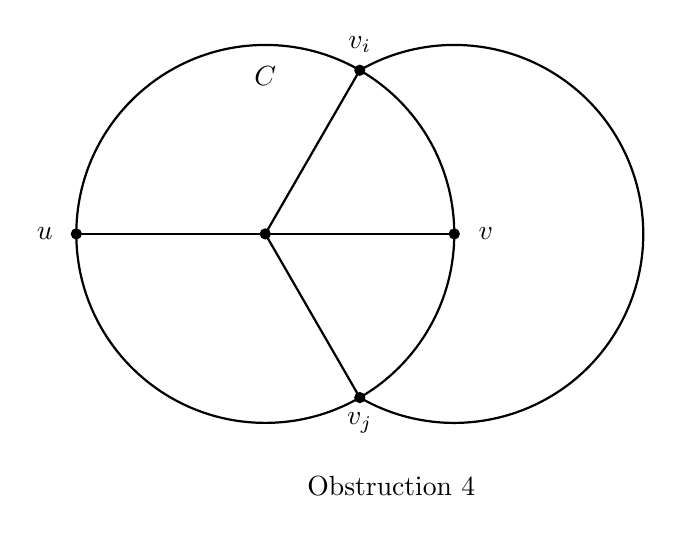
\begin{tikzpicture}[scale = 0.8]
            \draw[black, thick] (0,0) circle (3);
            \draw[black, thick] (1.5,-{sqrt(27/4)}) arc (-120:120:3);
            \draw[black, thick] (3,0) -- (-3,0);
            \draw[black, thick] (0,0) -- (1.5,{sqrt(27/4)});
            \draw[black, thick] (0,0) -- (1.5,-{sqrt(27/4)});
            \filldraw[black, thick] (-3,0) circle (2pt);
            \filldraw[black, thick] (3,0) circle (2pt);
            \filldraw[black, thick] (1.5,{sqrt(27/4)}) circle (2pt);
            \filldraw[black, thick] (1.5,-{sqrt(27/4)}) circle (2pt);
            \filldraw[black, thick] (0,0) circle (2pt);
            \node at (1.5,3,0) {$v_i$};
            \node at (1.5,-3,0) {$v_j$};
            \node at (-3.5,0,0) {$u$};
            \node at (3.5,0,0) {$v$};
            \node at (0,2.5,0) {$C$};

            \node at (2,-4,0) {Obstruction 4};
        \end{tikzpicture}
    \end{minipage}
    \hfill
    \begin{minipage}{0.4\textwidth}
        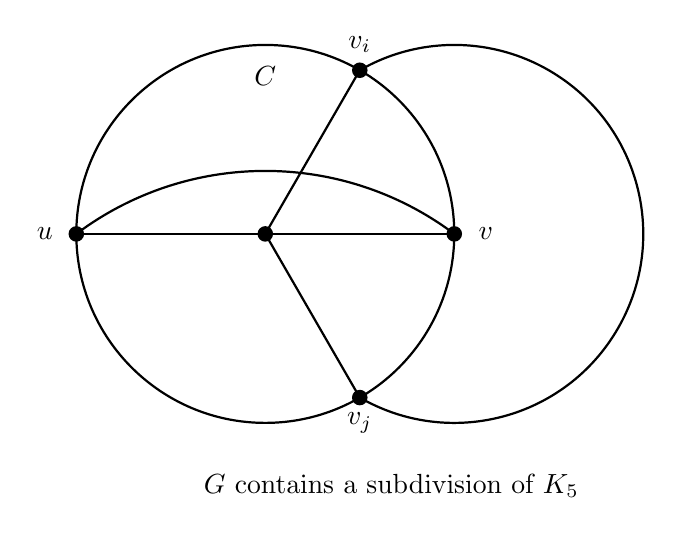
\begin{tikzpicture}[scale = 0.8]
            \draw[black, thick] (3,0) arc (acos(0.6):180-acos(0.6):5);
            \draw[black, thick] (0,0) circle (3);
            \draw[black, thick] (1.5,-{sqrt(27/4)}) arc (-120:120:3);
            \draw[black, thick] (3,0) -- (-3,0);
            \draw[black, thick] (0,0) -- (1.5,{sqrt(27/4)});
            \draw[black, thick] (0,0) -- (1.5,-{sqrt(27/4)});
            \filldraw[black, thick] (-3,0) circle (3pt);
            \filldraw[black, thick] (3,0) circle (3pt);
            \filldraw[black, thick] (1.5,{sqrt(27/4)}) circle (3pt);
            \filldraw[black, thick] (1.5,-{sqrt(27/4)}) circle (3pt);
            \filldraw[black, thick] (0,0) circle (3pt);
            \node at (1.5,3,0) {$v_i$};
            \node at (1.5,-3,0) {$v_j$};
            \node at (-3.5,0,0) {$u$};
            \node at (3.5,0,0) {$v$};
            \node at (0,2.5,0) {$C$};
            \node at (2,-4,0) {$G$ contains a subdivision of $K_5$};

        \end{tikzpicture}
    \end{minipage}
\end{figure}
\begin{remark}
    $G$ always contains a subgraph which is subdivisionof $K_5$ or $K_{3,3}$
\end{remark}
In all of the four cases the result is a 4 cases, the result is a contradiction. We assume that $G$ contained at neither of the two graphs. With this, we are left to conclude that there are no nonplanar graphs like $G$. This proves the theorem.
